\section{Baseline Performance}
\subsection{Our Framework}
We apply our automatic leaf segmentation, alignment, and tracking framework~\cite{yin2014a,yin2014b} to the Arabidopsis imagery to provide a baseline for future research.
Leaf segmentation aims at finding the correct number of leaves and the corresponding boundary of each leaf in each image.
Leaf alignment is to align the two tips of each leaf.
Leaf tracking is designed to track each leaf over time.

\begin{figure}[h]
\centering
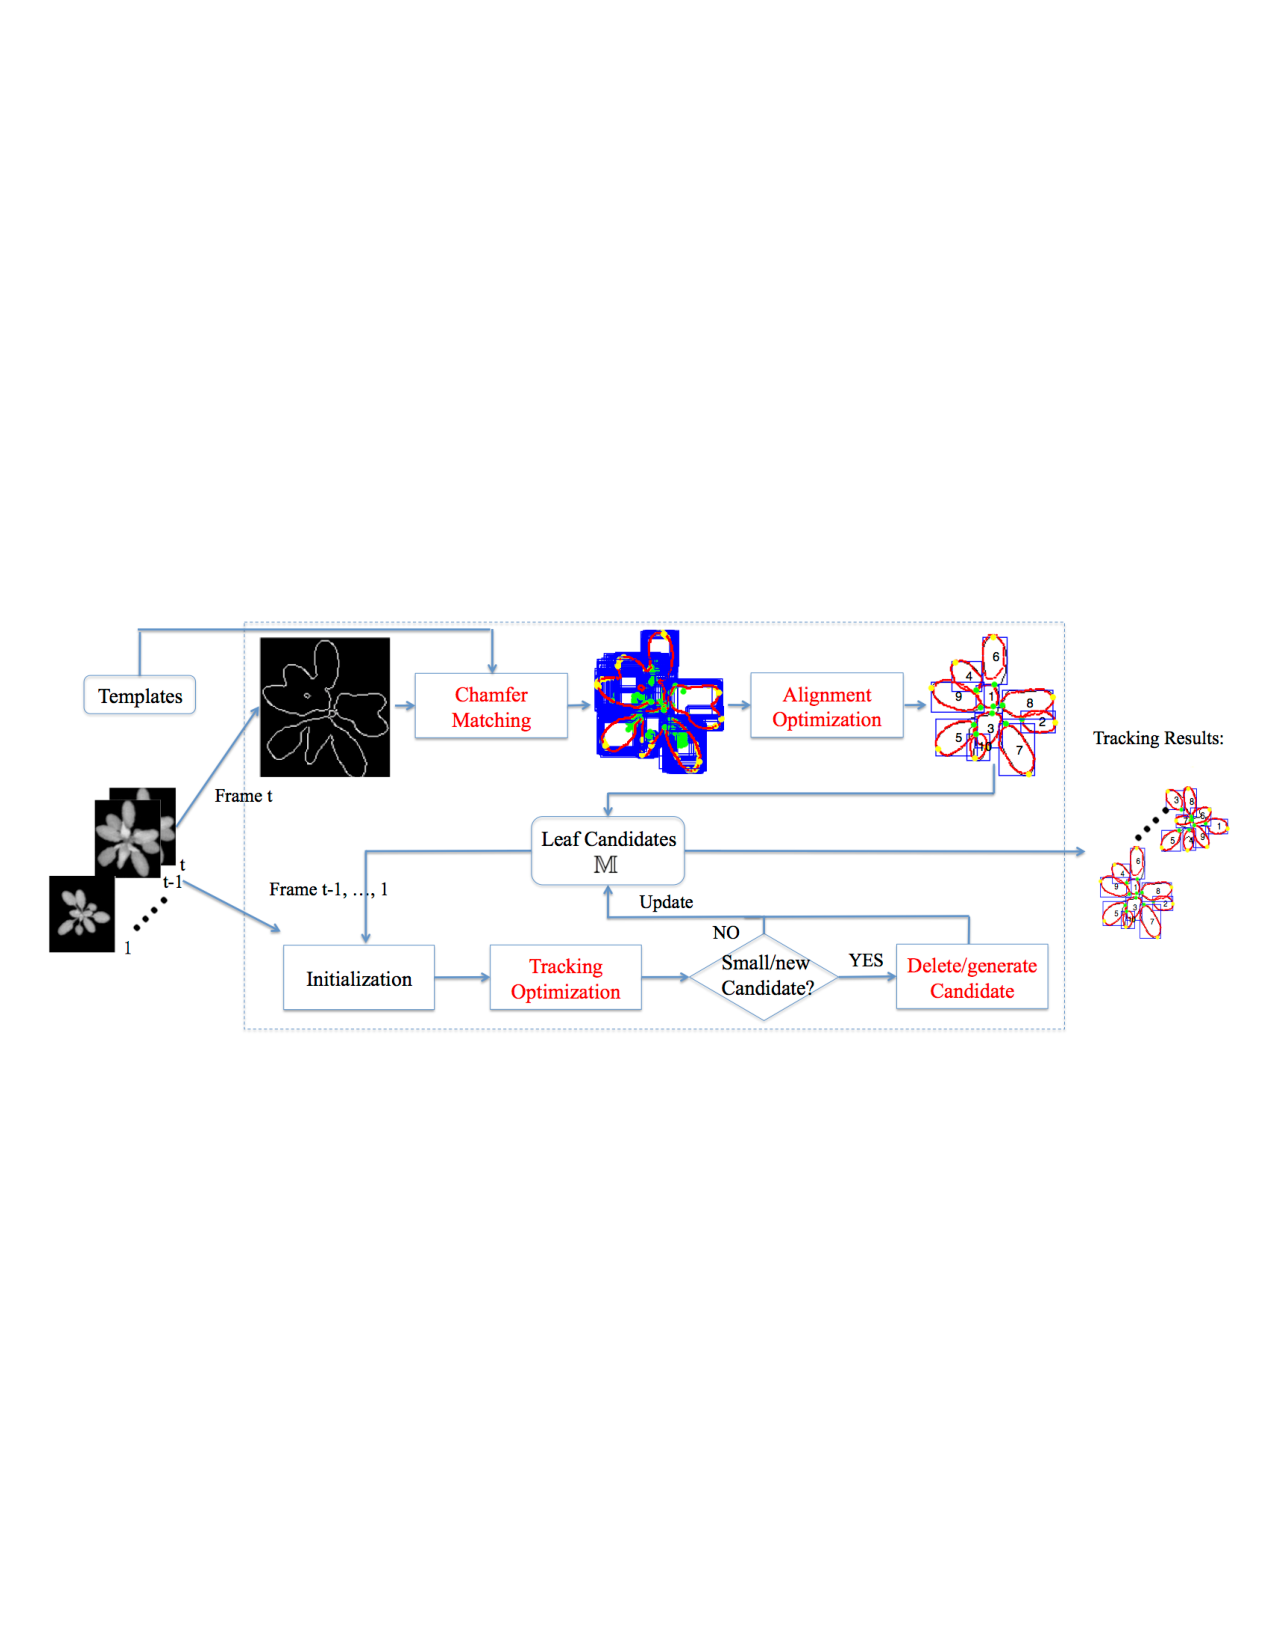
\includegraphics[width=.98\textwidth]{Figures/overview}\\
\caption{Overview of the baseline method.}
\label{fig:methodOverview}
\end{figure}

As shown in Fig~\ref{fig:methodOverview}, the input of this framework is a plant video and a set of predefined templates with various shapes, scales, and orientations.
We also generate the two tips for each template for finding the corresponding tip points of each leaf via Chamfer Matching~\
First, we apply multi-leaf alignment~\cite{yin2014a} approach to find an optimal set of leaf candidates on the last frame of the video, which will provide the information of the number of leaves, tip locations and boundaries of each leaf.
Second, we apply multi-leaf tracking~\cite{yin2014b} approach, which is based on leaf template transformation, to track leaves between continuous two frames.
In the tracking process, we develop a procedure to generate new leaves and delete small leaves. 
For each frame of the video, we can generate a label image with each leaf being labeled with one color and the tip locations for each piece of leaf. 
The label for each leaf in the video maintain the same during tracking process. 


\subsection{Performance Evaluation}
To evaluate the performance of leaf segmentation, alignment, and tracking, we use four criteria and provide the Matlab implementations.
Three of them are based on tip-based error, which is defined as average distance of a pair of estimated leaf tips $\hat{\bm{t}}_{1,2}$ with a pair of labeled leaf tips $ \bm{t}_{1,2}$ normalized by the labeled leaf length:

\begin {equation}
e_{la}(\hat{\bm{t}}_{1,2}, \bm{t}_{1,2}) = \frac{||\hat{\bm{t}}_1-{\bm{t}}_1||_2 + ||\hat{\bm{t}}_2-{\bm{t}}_2||_2}{2 ||\bm{t}_1-\bm{t}_2||_2}.
\label{eqn:tipError}
\end{equation}

We build the frame-to-frame and video-to-video correspondence respectively and generate two sets of tip-based errors.
More details can be find in~\cite{};
We define a threshold $\tau$ to operate on the corresponding tip-based errors. 
By varying $\tau$, we compute the first three criteria as:
\begin{itemize}
  \item {\it{Unmatched Leaf Rate(ULR)}}, the percentage of unmatched leaves w.r.t. the total number of labeled leaves. This can attribute to two sources. First, miss detections and false alarms. Second, matched leaves with tip-based errors larger than $\tau$.
  \item {\it{Landmark Error(LE)}}, the average tip-based errors smaller than $\tau$ of all frame-to-frame correspondent leaves.
  \item {\it{Tracking Consistency(TC)}}, the average tip-based errors smaller than $\tau$ of all video-to-video correspondent leaves. 
\end{itemize}

In order to evaluate the leaf segmentation accuracy, we adopt an additional metric~\cite{scharr2014annotated} based on the Dice score of estimated segmentation result and ground truth label:
\begin{itemize}
  \item {\it{Symmetric Best Dice(SBD)}}, the symmetric best Dice among all labeled leaves.
\end{itemize}

The results of our algorithm by varying $\tau$ from 0 to 1 is shown in Fig.XXX.
And the SBD score is XXX by averaging over all plants. 






